Quelques adresses utiles :
\begin{itemize}
\item[$\bullet$]le site de l'agrégation de mathématiques \url{http://agreg.org}, vous y trouverez des textes pour vous entraîner, et surtout les comptes rendus du jury. Aussi, la liste des logiciels acceptés à l'agreg : \textbf{Python, Scilab, Octave, Sage, Maxima, Xcas, R}. Tous sont libres et gratuits.
\item[$\bullet$]la page de la préparation de Rennes  \url{https://perso.univ-rennes1.fr/florent.malrieu/agreg-probas.html}
\end{itemize}

\section{Théorèmes limites dans le cas IID}

Les deux théorèmes suivant sont à maîtriser impérativement.

\begin{thm}[LGN et TCL]
Soient $X_1,...,X_n$ des variables aléatoires indépendantes identitquement distribuées, centrées et réduites, on note $\hat \theta_n =\frac{1}{n}\sum X_j$. Alors
\[\hat\theta_n\rightarrow _{ps}0,\]
\[\sqrt{n}\hat\theta_n\rightarrow _{\mathcal L}0.\] 
\end{thm}

Pour l'illustrer avec Scilab, on peut :\\

\begin{itemize}
\item[$\bullet$] tirer aléatoirement des variables aléatoires iid
\item[$\bullet$] calculer la moyenne empirique et montrer qu'elle converge vers l'espérance
\item[$\bullet$] répéter l'opération pour obtenir un échantillon de moyennes empiriques
\item[$\bullet$] tracer la fonction de répartition empirique, et montrer qu'elle converge en norme sup vers la fonction de répartition d'une normale. 
\item[$\bullet$] montrer que cela n'arrive pas avec certaines lois bien choisies. Par exemple la loi de Cauchy.\\
\end{itemize}

Un bon contre-exemple est la loi de Cauchy, de densité 
\[P(dx)=\frac{1}{\pi}\frac{1}{1+x^2}dx.\]
On voit qu'elle ne satisfait pas les hypothèses : elle n'a pas de moment d'ordre $1$, puisqu'équivalente à $\text{cte}.\frac{1}{x}$ en $+\infty$.\\ 
Pour la simuler, on peut utiliser le lemme suivant. 

\begin{lem}
Soit $X$ une variable aléatoire de fonction de répartition $F$ et $U$ suivant une loi uniforme sur l'intervalle $[0,1]$. Alors $F^{-1}(U)$ et $X$ ont mêmes lois.
\end{lem}

\begin{dem}
On rappelle que les fonctions de répartition sont caractérisées par les propriétés suivantes :
\begin{itemize}
\item[$\bullet$] $F$ est càd-làg (continue à droite limite à gauche),
\item[$\bullet$] $F$ est croissante,
\item[$\bullet$] $\lim_{-\infty} F =0$ et $\lim_\infty F =1$.
\end{itemize}
$F$ n'admet pas focément d'inverse, mais une inverse généralisée définie par 
\[F^{-1}(y) = \inf\{x : F(x)\leq y\}.\]
Alors :
\[P(F^{-1}(U)\leq x)= P(U\leq F(x)) = F(x).\]
\qed
\end{dem}
Pour, la loi de Cauchy, un simple calcul donne $F(x)=\frac{1}{\pi}\arctan(x)+\frac{1}{2}$, et $F^{-1}(u)=\tan(\pi(y-\frac{1}{2}))$. 

Le code suivant illustre cela, avec une fonction courte pour afficher des fonctions de répartition empiriques.\\

\fbox{\begin{minipage}{0.9\textwidth} 
N=500\\
m=10\\

\textbf{Loi normale, exponentielle, et de Cauchy}\\

Z=grand(1,N,'nor',0,1)\\
W= grand(1,N,'exp',2)\\
U=rand(1,N)\\
Cauchy=30*tan($\%$ pi*(U-0.5))\\

\textbf{Loi des grands nombres}
function esperance=esperance(X)\\
    [p,q]=size(X)\\
    scf()\\
    plot2d([1:q],cumsum(X)./[1:q],2)\\
    xtitle("Loi des grands nombres" )\\
endfunction\\

esperance(Z)\\
plot2d([0:N],0*[0:N])\\

\textbf{FDR empirique}

$//$ Theoreme Central Limite\\
function plotFDR=plotFDR(X)\\
 \quad     [p,q]=size(X);\\
  \quad    scf()\\
 \quad     plot2d2(-sort(-X),(1/q)*[1:q],2)\\
 \quad     xtitle("Fonction de repartition empirique")\\
endfunction\\

h=0.1;\\
t=[-5:h:5];\\

plotFDR(Z)\\
ynor=cdfnor("PQ",t,0*t,0*t+1)\\
plot2d(t,ynor)\\

plotFDR(W)\\
t=[0:h:5];\\
ypoi=cdfpoi("PQ",t,0*t+2)\\
plot2d(t,ypoi)\\

plotFDR(Cauchy)\\
\end{minipage}}\\
\\

\section{Chaînes de Markov}

On rappelle qu'une chaîne de Marov est l'analogue probabiliste d'une suite récurrente d'ordre $1$. C'est la donnée d'un couple $(E,P)$ où $E$ est un espace d'état, et $P : E\times E\rightarrow [0,1]$ un noyau de transition.\\

Vous devez connaître ces définitions, ainsi que
\begin{itemize}
\item[$\bullet$] la définition de la propriété de Markov
\item[$\bullet$] l'équation de Chapman-Kolmogorov
\item[$\bullet$] la définition de mesure invariante $\nu P =\nu$, de mesure réversible $\nu(x)P(x,y)=\nu(y)P(y,x)$, et savoir montrer que réversible entraîne invariante.\\
\end{itemize}

Supposons que l'espace d'états $E$ est fini. Alors l'espace des probabilités invariantes est un compact convexe non-vide du simplexe des probabilités sur $E$, vue comme un sous-espace de $\R^{|E|}$. En particulier, il existe une mesure invariante. Pour l'unicité, il suffit que la chaîne soit irréductible, i.e. que le graphe de transition soit connexe. 

\begin{thm}[Théorème ergodique]
Si $(X_n)$ une trajectoire d'une chaîne de Markov irréductible, d'unique probabilité invariante $\nu$. Alors pour toute fonction $\phi :E\rightarrow \R$, 
\[\frac{1}{n}\sum_{k=1}^n \phi(X_k) \rightarrow \int_E \phi(x)\nu(dx).\]
Alors \[\nu(x)=\frac{1}{E[T_x]},\]
où $T_x=\inf\{n>1 : X_n = x\}$ est le temps de retour en $x$.\\
De plus, si la chaîne est fortement apériodique, alors on a, pour toute mesure de probabilité initiale $\mu_0$, la convergence en loi suivante :
\[\mu_0 P^n \rightarrow \nu, \]
i.e. $(X_n)_n$ converge en loi vers $\nu$ quelle que soit sa distribution initiale.
\end{thm}

Vous devez penser à la mesure invariante comme la mesure que le système atteint à l'équilibre. Par exemple, dans le modèle de l'urne d'Ehrenfest, on avait $E=\{0,1,2,...,m\}$, 
\[P(k,k-1)=1-P(k,k+1)=\frac{k}{m} \quad \text{et}\quad P(0,1)=P(m,m-1)=1.\]
Ce modèle est sensé représenter $m$ particules indistingables dans une pièce, que l'on sépare en deux zones distinctes $A$ et $B$. L'état du système est entièrement determiné par le nombre $X_T$ de particules qui se trouvent à l'instant $T$ dans la zone $A$ par exemple.\\

La chaîne est irréductible, mais admet une période : la parité des états vistés alterne en fonction du temps. On ne peut donc qu'appliquer la convergence presque-sûre, et pas la convergence en loi, dans le théorème ergodique.\\

Un simple calcul montre que $\nu(x)=\frac{1}{2^m}\binom{x}{m}$ est une mesure réversible, donc invariante, qui est unique par irréductibilité. Cela signifie que si l'expérimentateur lance son expérience, quitte la pièce assez longtemps pour que le système atteigne l'équilibre, et qu'il fait une mesure du nombre de particules dans la zone $A$ lors de son retour, il trouvera $x$ avec une probabilité proche de $\nu(x)$ (d'autant plus proche que le temps passe).\\

Un point inquiétant du modèle est qu'il autorise un retour à l'état $0$ ou $m$, ce qui siginifie que toute les particules de la pièce sont concentrées dans une partie de la pièce, laissant l'autre vide. Si le jury soulève cette question, vous pouvez alors utiliser le théorème ergodique pour arguer que le temps de retour :\\

\begin{itemize}
\item[$\bullet$] en $m$ est de l'ordre de 
\[E[T_m]=\frac{1}{\nu(m)}=\frac{1}{2^m} \]
\item[$\bullet$] en $\frac{m}{2}$ est de l'ordre de 
\[E[T_{m/2}]=\frac{1}{\nu(m/2)}\sim\sqrt{\frac{\pi m}{2}} \]
en utilisant la formule de Stirling.\\
\end{itemize}

Le nombre $m$ étant supposé très grand, il faudrait à l'expérimentateur attendre très longtemps pour voir se réaliser une situation pareille. Enfin, si on note $Z$ une normale centrée réduite :
\[\nu([\frac{m}{2}\pm 2\epsilon \sqrt{m}]) \simeq P(|Z|>\epsilon)=1-2P(Z>\epsilon) \]
et 
\[P(Z>\epsilon)=P(e^{tZ}>e^{t\epsilon})\leq \frac{E[e^{tZ}]}{(t\epsilon)^2}.\]
Ce calcul montre que toute la masse de la mesure invariante est concentrée autour de l'état $m/2$, i.e. qu'à l'équilibre, un expérimentateur ne peut mesurer qu'un nombre de particules pratiquement égal dans les deux zones (avec une très forte probabilité).\\

Le calcul utilise successivement :
\begin{itemize}
\item[$\bullet$] l'approximation gaussienne de la binomiale,
\item[$\bullet$] la symmétrie de la loi normale,
\item[$\bullet$] l'inégalité de Markov.
\end{itemize}

Voici pour la simulation. Essentiellement, on entrela matrice de transition, et on utilise l'option \textit{markov} de \textit{grand}.\\

\fbox{\begin{minipage}{0.9\textwidth} 
//Entree de la matrice de transition de la chaine de Markov associee au modele d Ehrenfest\\

function P=ehrenfest(N)\\
d1=(N-(0:N-1))/N;\\
d2=(1:N)/N;\\
P=diag(d1,1)+diag(d2,-1);\\
endfunction;\\

// Simulation\\
m=1000\\
T=100000\\
x0=m\\
X=grand(T,'markov',ehrenfest(m),x0)\\
plot([1:T],X)\\
\end{minipage}}\\
\\

On peut facilement voir que le système atteint rapidement l'état d'équilibre sur la figure ~\ref{Ehrenfest}. C'est un fait général : la vitesse de convergence est dominé par le plus grand module $<1$ des valeurs propres de la matrice de transition $P$. Cela est donné par le théorème de Perron-Frobenius.

\begin{figure}[h]\centering
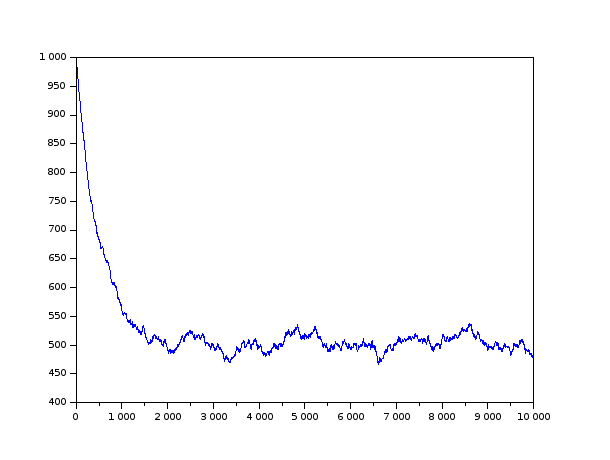
\includegraphics[scale=0.4]{Ehrenfest.png}
\caption{Une trajectoire partant de l'état $m=1000$ particules dans la zone $A$}
\label{fig:Ehrenfest}
\end{figure}









